\documentclass{article}
\usepackage{blindtext}
\usepackage{booktabs}
\usepackage[margin=0.25in]{geometry}
\usepackage{subcaption}
\usepackage{graphicx}
\usepackage{caption}
\usepackage{hyperref}
\usepackage{pdflscape}
\usepackage{tikz}
\usepackage{threeparttable}
\usepackage{algorithmic}
\usepackage{tabularx}

\title{New ssaggregate tables}

\begin{document}
\maketitle
\tableofcontents
{\footnotesize 
\listoffigures
\listoftables}
\clearpage

\section{Main Updates}
\begin{landscape}
\begin{table}[htbp]\centering \def\sym#1{\ifmmode^{#1}\else\(^{#1}\)\fi}  \begin{threeparttable} \caption{Total Black Balance}
\footnotesize
 \begin{tabular}{l*{2}{c}} \toprule
                &\multicolumn{1}{c}{$\widehat{GM}$}\\
\midrule
Average precipitation&   -0.046   \\
                &  (0.391)   \\
\addlinespace
Average temperature&   -0.821   \\
                &  (1.357)   \\
\addlinespace
Coastal CZ      &    0.001   \\
                &  (0.017)   \\
\addlinespace
Share of LF employed in manufacturing, 1940&    1.177** \\
                &  (0.468)   \\
\addlinespace
Meters of Railroad per Square Meter of Area, 1940&    0.000   \\
                &  (0.000)   \\
\addlinespace
Average Transport Cost out of CZ, 1920&   -0.047   \\
                &  (0.038)   \\
\addlinespace
Fraction of area incorporated&    0.015   \\
                &  (0.010)   \\
\addlinespace
Prop HS Grads   &   -0.005   \\
                &  (0.003)   \\
\addlinespace
Prop College Grads&   -0.003   \\
                &  (0.003)   \\
\addlinespace
Average Income (1940)&   15.334*  \\
                &  (8.076)   \\
\addlinespace
Population Density, 1940&   22.346*  \\
                & (11.898)   \\
\addlinespace
1930-40 Population Growth Rate&   -0.038   \\
                &  (0.389)   \\
       \bottomrule \end{tabular}

\end{threeparttable}  \end{table}
\clearpage




\begin{table}[htbp]\centering \def\sym#1{\ifmmode^{#1}\else\(^{#1}\)\fi}  \begin{threeparttable} \caption{Main Results, Black}
\footnotesize
\input{tables/final/black_ssaggregate.tex}
\end{threeparttable}  \end{table}
\clearpage

\begin{table}[htbp]\centering \def\sym#1{\ifmmode^{#1}\else\(^{#1}\)\fi}  \begin{threeparttable} \caption{2010 Results, Black}
\footnotesize
 \begin{tabularx}{\textwidth}{l*{6}{>{\centering\arraybackslash}X}} \toprule \setlength{\tabcolsep}{15pt}
&\multicolumn{1}{c}{C. Goodman}&\multicolumn{4}{c}{Census of Governments}&\multicolumn{1}{c}{Census}\\\cmidrule(lr){2-2}\cmidrule(lr){3-6}\cmidrule(lr){7-7}
&\multicolumn{2}{c}{Municipalities}&\multicolumn{1}{c}{School districts}&\multicolumn{1}{c}{Townships}&\multicolumn{1}{c}{Special districts}&\multicolumn{1}{c}{Main City Share}\\\cmidrule(lr){2-3}\cmidrule(lr){4-6}\cmidrule(lr){7-7}
&\multicolumn{1}{c}{(1)}&\multicolumn{1}{c}{(2)}&\multicolumn{1}{c}{(3)}&\multicolumn{1}{c}{(4)}&\multicolumn{1}{c}{(5)}&\multicolumn{1}{c}{(6)}\\
\cmidrule(lr){1-7}
\multicolumn{6}{l}{Panel A: First Stage}\\
\cmidrule(lr){1-7}
(sum) shift\_share&    1.771***&    1.771***&    1.841***&    1.771***&    1.771***&    1.771***\\
                &  (0.315)   &  (0.315)   &  (0.330)   &  (0.315)   &  (0.315)   &  (0.315)   \\
\cmidrule(lr){1-7}
\multicolumn{6}{l}{Panel B: OLS}\\
\cmidrule(lr){1-7}
GM\_raw\_pp       &    0.005   &    0.007   &    0.101   &    0.021***&   -0.009   &   -1.137***\\
                &  (0.005)   &  (0.005)   &  (0.077)   &  (0.007)   &  (0.008)   &  (0.223)   \\
\cmidrule(lr){1-7}
\multicolumn{6}{l}{Panel C: Reduced Form}\\
\cmidrule(lr){1-7}
(sum) shift\_share&    0.018   &    0.021   &    0.327   &    0.079***&    0.035   &   -3.317***\\
                &  (0.013)   &  (0.015)   &  (0.285)   &  (0.026)   &  (0.031)   &  (0.639)   \\
\cmidrule(lr){1-7}
\multicolumn{6}{l}{Panel D: 2SLS}\\
\cmidrule(lr){1-7}
GM\_raw\_pp       &    0.010*  &    0.012*  &    0.178** &    0.045***&    0.020***&   -1.873***\\
                &  (0.005)   &  (0.006)   &  (0.086)   &  (0.006)   &  (0.005)   &  (0.161)   \\
\midrule
First Stage F-Stat&    31.55   &    31.55   &    31.18   &    31.55   &    31.55   &    31.55   \\
Dep. Var. Mean  &    -0.39   &    -0.49   &   -13.31   &    -0.86   &     1.04   &    -7.96   \\
1940 Dep. Var. Mean&     1.49   &     1.61   &    14.09   &     2.29   &     0.89   &    32.86   \\
Observations    &      130   &      130   &      118   &      130   &      130   &      130   \\
 \bottomrule \end{tabularx}

\end{threeparttable}  \end{table}
\clearpage


\begin{figure}
	\centering
	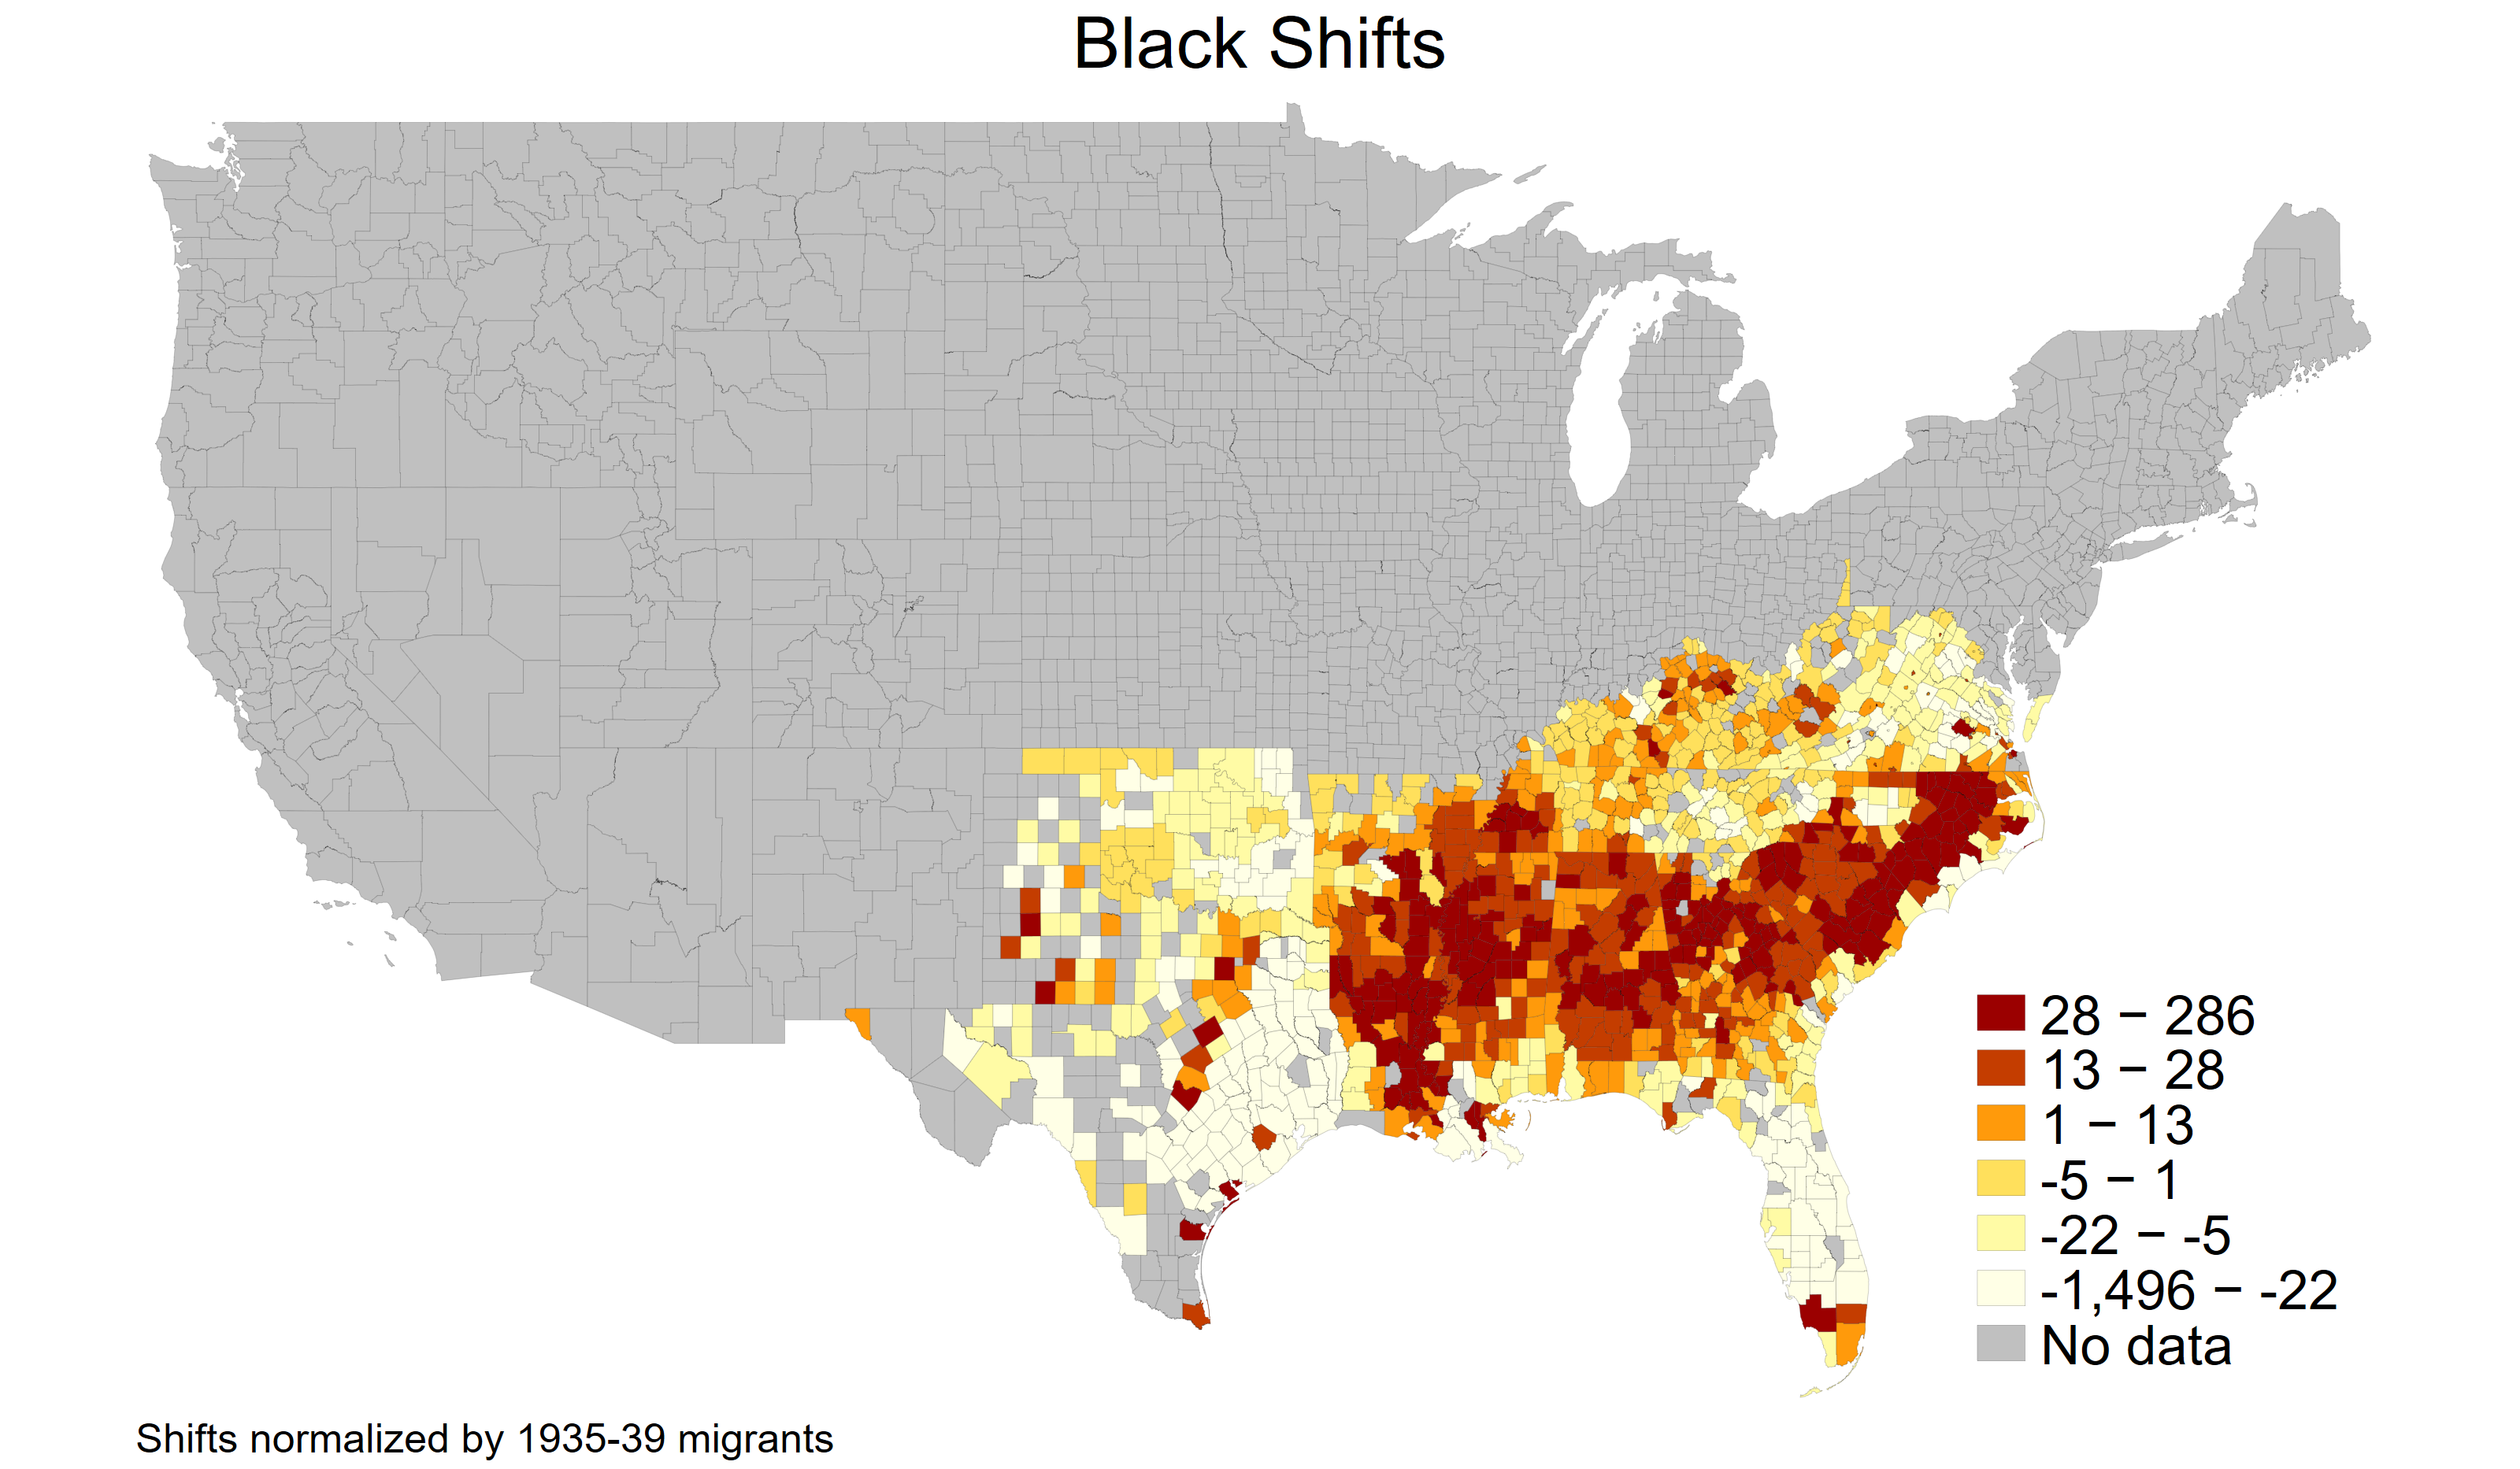
\includegraphics[width=0.9\linewidth]{figures/base_shifts.png}
\end{figure}
\clearpage

\section{White Instrument}

\begin{table}[htbp]\centering \def\sym#1{\ifmmode^{#1}\else\(^{#1}\)\fi}  \begin{threeparttable} \caption{Total White  Balance}
\footnotesize
\begin{tabular}{l*{3}{c}} \toprule
&\multicolumn{2}{c}{$\widehat{WM}$}&\multicolumn{1}{c}{Mean}\\\cmidrule(lr){2-3}\cmidrule(lr){4-4}
&\multicolumn{1}{c}{(1)}&\multicolumn{1}{c}{(2)}&\multicolumn{1}{c}{(3)}\\
\midrule 
Average precipitation  &    0.161 & 0.159 & 15.069 \\
                &  (0.530)  &  (0.522)  &  (13.966)    \\
Average temperature  &    0.143 & 0.474 & 40.212 \\
                &  (1.055)  &  (1.111)  &  (18.626)    \\
Number of Streams  &    23.954 & 23.673 & 496.864 \\
                &  (21.282)  &  (23.280)  &  (346.704)    \\
Coastal CZ  &    -0.029** & -0.034** & 0.491 \\
                &  (0.012)  &  (0.014)  &  (0.502)    \\
Share of LF employed in manufacturing, 1940  &    1.181** & 1.507*** & 25.027 \\
                &  (0.587)  &  (0.409)  &  (8.409)    \\
Meters of Railroad per Square Meter of Area, 1940  &    0.000 & 0.000 & 0.000 \\
                &  (0.000)  &  (0.000)  &  (0.000)    \\
Average Transport Cost out of CZ, 1920  &    -0.040 & -0.037 & 9.575 \\
                &  (0.030)  &  (0.028)  &  (2.684)    \\
Fraction of area incorporated  &    -0.019* & -0.018* & 0.212 \\
                &  (0.010)  &  (0.011)  &  (0.225)    \\
Prop HS Grads, (25+)  &    -0.010*** & -0.013*** & 0.263 \\
                &  (0.003)  &  (0.002)  &  (0.058)    \\
Prop College Grads, (25+)  &    -0.003*** & -0.004*** & 0.054 \\
                &  (0.001)  &  (0.001)  &  (0.012)    \\
Average Income, 1940  &    -16.171** & -17.130** & 1163.364 \\
                &  (7.159)  &  (7.610)  &  (91.873)    \\
Population Density, 1940  &    -15.366 & -13.090 & 257.039 \\
                &  (12.492)  &  (12.727)  &  (281.115)    \\
1930-40 Population Growth Rate  &    -0.004 & -0.011*** & 0.076 \\
                &  (0.007)  &  (0.003)  &  (0.073)    \\
\bottomrule \end{tabular}

\end{threeparttable}  \end{table}
\clearpage

\begin{table}[htbp]\centering \def\sym#1{\ifmmode^{#1}\else\(^{#1}\)\fi}  \begin{threeparttable} \caption{Main Results, White}
\footnotesize
\input{tables/final/white_ssaggregate.tex}
\end{threeparttable}  \end{table}
\clearpage



\begin{table}[htbp]\centering \def\sym#1{\ifmmode^{#1}\else\(^{#1}\)\fi}  \begin{threeparttable} \caption{2010 Results, White}
\footnotesize
 \begin{tabularx}{\textwidth}{l*{6}{>{\centering\arraybackslash}X}} \toprule \setlength{\tabcolsep}{15pt}
&\multicolumn{1}{c}{C. Goodman}&\multicolumn{4}{c}{Census of Governments}&\multicolumn{1}{c}{Census}\\\cmidrule(lr){2-2}\cmidrule(lr){3-6}\cmidrule(lr){7-7}
&\multicolumn{2}{c}{Municipalities}&\multicolumn{1}{c}{School districts}&\multicolumn{1}{c}{Townships}&\multicolumn{1}{c}{Special districts}&\multicolumn{1}{c}{Main City Share}\\\cmidrule(lr){2-3}\cmidrule(lr){4-6}\cmidrule(lr){7-7}
&\multicolumn{1}{c}{(1)}&\multicolumn{1}{c}{(2)}&\multicolumn{1}{c}{(3)}&\multicolumn{1}{c}{(4)}&\multicolumn{1}{c}{(5)}&\multicolumn{1}{c}{(6)}\\
\cmidrule(lr){1-7}
\multicolumn{6}{l}{Panel A: First Stage}\\
\cmidrule(lr){1-7}
(sum) shift\_share&    1.185***&    1.185***&    0.694   &    1.185***&    1.185***&    1.185***\\
                &  (0.412)   &  (0.412)   &  (0.495)   &  (0.412)   &  (0.412)   &  (0.412)   \\
\cmidrule(lr){1-7}
\multicolumn{6}{l}{Panel B: OLS}\\
\cmidrule(lr){1-7}
WM\_raw\_pp       &   -0.004   &   -0.005   &   -0.162** &   -0.018** &    0.013*  &    1.062***\\
                &  (0.005)   &  (0.005)   &  (0.063)   &  (0.009)   &  (0.008)   &  (0.205)   \\
\cmidrule(lr){1-7}
\multicolumn{6}{l}{Panel C: Reduced Form}\\
\cmidrule(lr){1-7}
(sum) shift\_share&   -0.028** &   -0.034** &   -0.082   &   -0.047*  &   -0.041   &    1.866** \\
                &  (0.014)   &  (0.016)   &  (0.328)   &  (0.024)   &  (0.033)   &  (0.891)   \\
\cmidrule(lr){1-7}
\multicolumn{6}{l}{Panel D: 2SLS}\\
\cmidrule(lr){1-7}
WM\_raw\_pp       &   -0.024** &   -0.029** &   -0.118   &   -0.039***&   -0.035***&    1.574***\\
                &  (0.009)   &  (0.011)   &  (0.328)   &  (0.008)   &  (0.012)   &  (0.298)   \\
\midrule
First Stage F-Stat&     8.26   &     8.26   &     1.97   &     8.26   &     8.26   &     8.26   \\
Dep. Var. Mean  &    -0.39   &    -0.49   &   -13.31   &    -0.86   &     1.04   &    -7.96   \\
1940 Dep. Var. Mean&     1.49   &     1.61   &    14.09   &     2.29   &     0.89   &    32.86   \\
Observations    &      130   &      130   &      118   &      130   &      130   &      130   \\
 \bottomrule \end{tabularx}

\end{threeparttable}  \end{table}
\clearpage



\begin{figure}
	\centering
	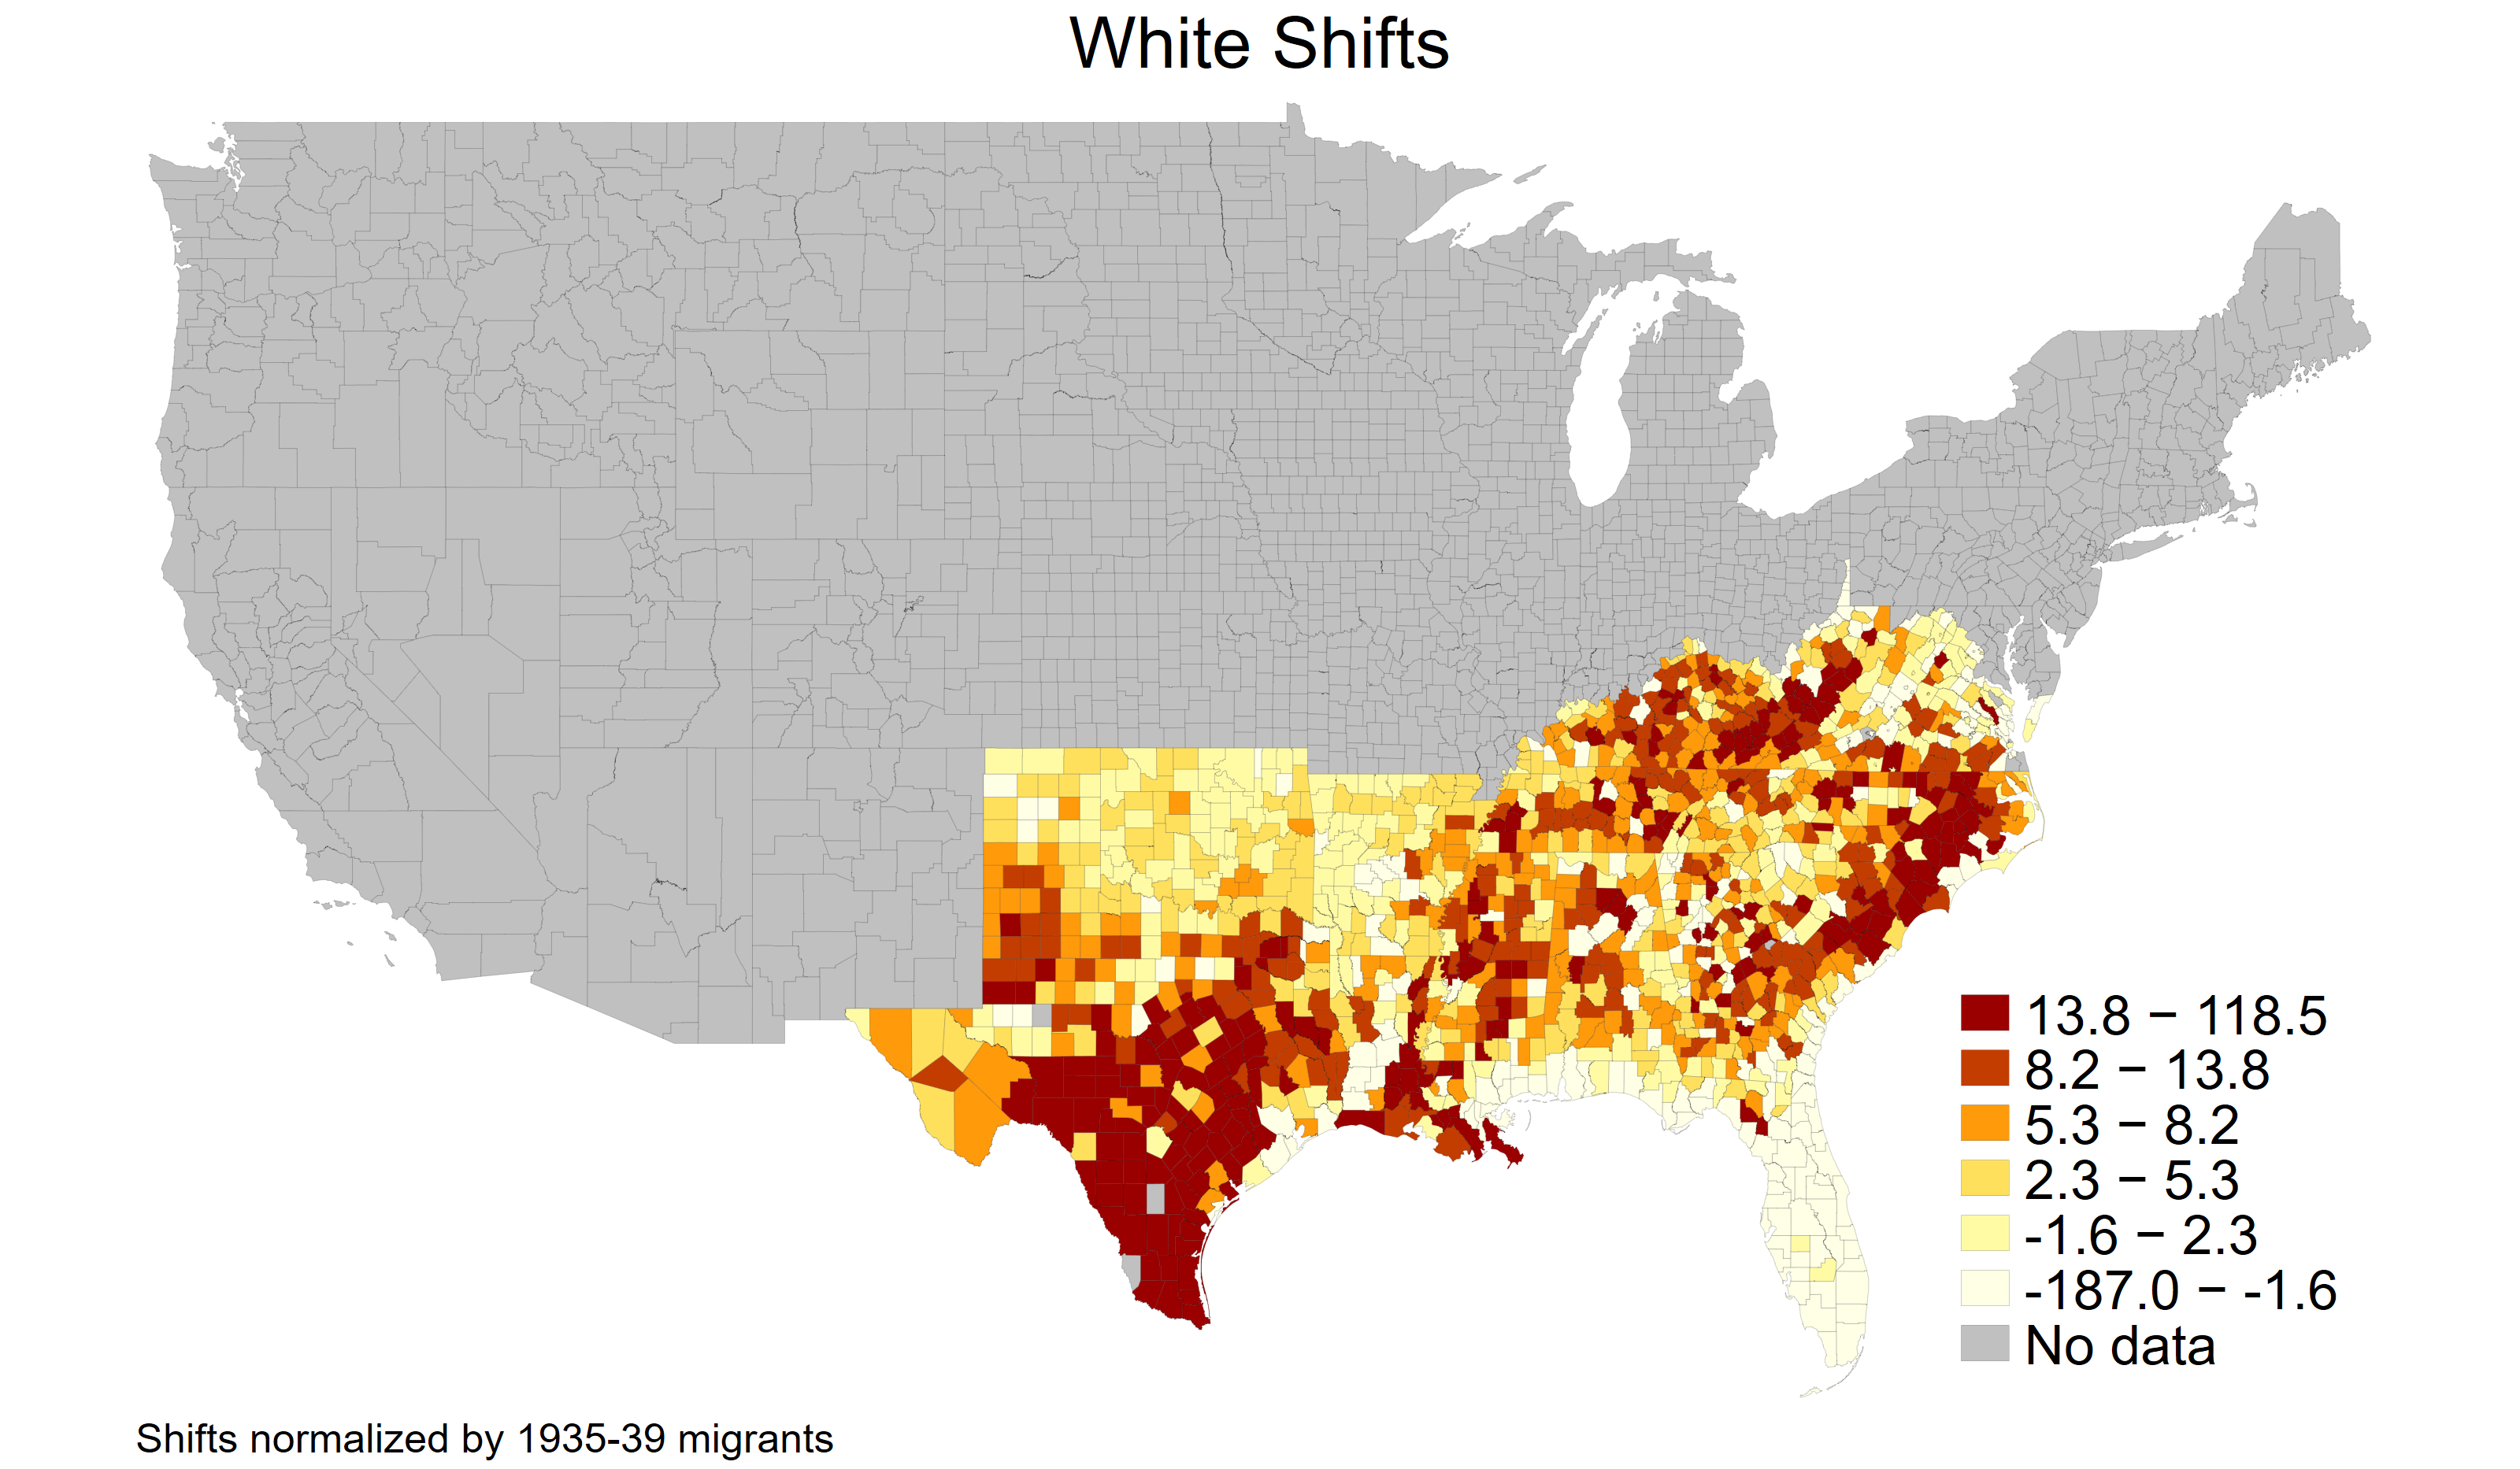
\includegraphics[width=0.9\linewidth]{figures/base_white_shifts.png}
\end{figure}
\clearpage


\section{Dropping Texas}
\begin{table}[htbp]\centering \def\sym#1{\ifmmode^{#1}\else\(^{#1}\)\fi}  \begin{threeparttable} \caption{Black Balance, No Texas}
\footnotesize
 \begin{tabular}{l*{2}{c}} \toprule
                &\multicolumn{1}{c}{$\widehat{GM}$}\\
\midrule
Average precipitation&   -0.926** \\
                &  (0.395)   \\
\addlinespace
Average temperature&   -2.497*  \\
                &  (1.455)   \\
\addlinespace
Coastal CZ      &    0.014   \\
                &  (0.013)   \\
\addlinespace
Share of LF employed in manufacturing, 1940&    1.656***\\
                &  (0.564)   \\
\addlinespace
Meters of Railroad per Square Meter of Area, 1940&    0.000   \\
                &  (0.000)   \\
\addlinespace
Average Transport Cost out of CZ, 1920&   -0.021   \\
                &  (0.037)   \\
\addlinespace
Fraction of area incorporated&    0.012   \\
                &  (0.012)   \\
\addlinespace
Prop HS Grads   &   -0.007   \\
                &  (0.005)   \\
\addlinespace
Prop College Grads&   -0.005   \\
                &  (0.005)   \\
\addlinespace
Average Income (1940)&   15.180   \\
                &  (9.532)   \\
\addlinespace
Population Density, 1940&   22.110   \\
                & (14.271)   \\
\addlinespace
1930-40 Population Growth Rate&    0.024   \\
                &  (0.412)   \\
       \bottomrule \end{tabular}

\end{threeparttable}  \end{table}
\clearpage

\begin{table}[htbp]\centering \def\sym#1{\ifmmode^{#1}\else\(^{#1}\)\fi}  \begin{threeparttable} \caption{White Balance, No Texas}
\footnotesize
 \begin{tabular}{l*{2}{c}} \toprule
                &\multicolumn{1}{c}{$\widehat{WM}$}\\
\midrule
Average precipitation&    0.458   \\
                &  (0.492)   \\
\addlinespace
Average temperature&    1.113   \\
                &  (1.093)   \\
\addlinespace
Coastal CZ      &   -0.032** \\
                &  (0.013)   \\
\addlinespace
Share of LF employed in manufacturing, 1940&    1.404***\\
                &  (0.440)   \\
\addlinespace
Meters of Railroad per Square Meter of Area, 1940&    0.000   \\
                &  (0.000)   \\
\addlinespace
Average Transport Cost out of CZ, 1920&   -0.038   \\
                &  (0.038)   \\
\addlinespace
Fraction of area incorporated&   -0.016*  \\
                &  (0.009)   \\
\addlinespace
Prop HS Grads   &   -0.003   \\
                &  (0.002)   \\
\addlinespace
Prop College Grads&    0.002   \\
                &  (0.001)   \\
\addlinespace
Average Income (1940)&  -11.372   \\
                &  (7.921)   \\
\addlinespace
Population Density, 1940&  -12.484   \\
                & (11.098)   \\
\addlinespace
1930-40 Population Growth Rate&   -1.248***\\
                &  (0.233)   \\
       \bottomrule \end{tabular}

\end{threeparttable}  \end{table}
\clearpage
\begin{table}[htbp]\centering \def\sym#1{\ifmmode^{#1}\else\(^{#1}\)\fi}  \begin{threeparttable} \caption{Main Results, Black, Texas Dropped}
\footnotesize
\input{tables/final/black_notx_ssaggregate.tex}
\end{threeparttable}  \end{table}
\clearpage


\begin{table}[htbp]\centering \def\sym#1{\ifmmode^{#1}\else\(^{#1}\)\fi}  \begin{threeparttable} \caption{Main Results, White, Texas Dropped}
\footnotesize
 \begin{tabularx}{\textwidth}{l*{6}{>{\centering\arraybackslash}X}} \toprule \setlength{\tabcolsep}{15pt}
&\multicolumn{1}{c}{C. Goodman}&\multicolumn{4}{c}{Census of Governments}&\multicolumn{1}{c}{Census}\\\cmidrule(lr){2-2}\cmidrule(lr){3-6}\cmidrule(lr){7-7}
&\multicolumn{2}{c}{Municipalities}&\multicolumn{1}{c}{School districts}&\multicolumn{1}{c}{Townships}&\multicolumn{1}{c}{Special districts}&\multicolumn{1}{c}{Main City Share}\\\cmidrule(lr){2-3}\cmidrule(lr){4-6}\cmidrule(lr){7-7}
&\multicolumn{1}{c}{(1)}&\multicolumn{1}{c}{(2)}&\multicolumn{1}{c}{(3)}&\multicolumn{1}{c}{(4)}&\multicolumn{1}{c}{(5)}&\multicolumn{1}{c}{(6)}\\
\cmidrule(lr){1-7}
\multicolumn{6}{l}{Panel A: First Stage}\\
\cmidrule(lr){1-7}
(sum) shift\_share&    1.184*  &    1.184*  &    0.350   &    1.184*  &    1.184*  &    1.184*  \\
                &  (0.604)   &  (0.604)   &  (0.423)   &  (0.604)   &  (0.604)   &  (0.604)   \\
\cmidrule(lr){1-7}
\multicolumn{6}{l}{Panel B: OLS}\\
\cmidrule(lr){1-7}
WM\_raw\_pp       &   -0.002   &   -0.004   &   -0.191***&   -0.016***&    0.011   &    0.729***\\
                &  (0.002)   &  (0.003)   &  (0.069)   &  (0.004)   &  (0.007)   &  (0.128)   \\
\cmidrule(lr){1-7}
\multicolumn{6}{l}{Panel C: Reduced Form}\\
\cmidrule(lr){1-7}
(sum) shift\_share&   -0.017   &   -0.024*  &   -0.069   &   -0.033   &   -0.012   &    1.194*  \\
                &  (0.011)   &  (0.015)   &  (0.307)   &  (0.021)   &  (0.025)   &  (0.696)   \\
\cmidrule(lr){1-7}
\multicolumn{6}{l}{Panel D: 2SLS}\\
\cmidrule(lr){1-7}
WM\_raw\_pp       &   -0.015   &   -0.021   &   -0.198   &   -0.028***&   -0.010   &    1.009***\\
                &  (0.010)   &  (0.013)   &  (0.483)   &  (0.009)   &  (0.011)   &  (0.219)   \\
\midrule
First Stage F-Stat&     3.84   &     3.84   &     0.68   &     3.84   &     3.84   &     3.84   \\
Dep. Var. Mean  &    -0.26   &    -0.33   &   -12.95   &    -0.57   &     0.64   &    -3.37   \\
1940 Dep. Var. Mean&     1.49   &     1.61   &    14.09   &     2.29   &     0.89   &    32.86   \\
Observations    &      130   &      130   &      118   &      130   &      130   &      130   \\
 \bottomrule \end{tabularx}

\end{threeparttable}  \end{table}
\clearpage


\end{landscape}
\end{document}
